\documentclass[a4paper,12pt]{article}
\usepackage[utf8]{inputenc}
\usepackage{graphicx}
\usepackage{float}
\usepackage[superscript]{cite}
\usepackage{color}


\usepackage{listings}
\definecolor{light-gray}{gray}{0.95}
\lstdefinestyle{normal}{
  basicstyle=\footnotesize\ttfamily,
  numbers=none,
  backgroundcolor=\color{light-gray},
  showspaces=false,
  showstringspaces=false,
  showtabs=false,
  tabsize=2,
  captionpos=b,
  escapechar=¤,
  frame=single,
  framesep=0.2cm,
  xleftmargin=2mm,
  xrightmargin=2mm,
  breaklines=true,
  emph={}
}
\lstset{style=normal}
\lstdefinestyle{javascript}{ language=JavaScript }
\lstdefinestyle{haskell}{ language=Haskell }
\lstset{style=haskell}

\title{HQMp3 -- MP3 decoder in Haskell}
\author{Tobias Olausson \\ \texttt{\small{olaussot@student.chalmers.se}} \and
        Anders Karlsson \\ \texttt{\small{andekar@student.chalmers.se}}
}
\date{ \rule{0.8 \linewidth}{0.5mm} \\[3mm]
       University of Gothenburg \\
       \small{\today}
}

\begin{document}
\maketitle

\begin{abstract}
    This project aims to show how one can parse and decode binary formats in
    Haskell, showcased by implementing an mp3 decoder. The decoder features its
    own library for handling of binary formats, a fast huffman decoder and is
    written entirely in Haskell. The project was carried out as a 15hp course at
    the department of computer science and engineering at the University of
    Gothenburg during the autumn 2009. 
\end{abstract}

\tableofcontents

\section{Motivation}
    MP3 decoders exists today in most languages, however there does not exist
    a fast one written in Haskell. It does exists one written by Björn Edström
    \cite{bjorn}, but it is very slow, and partly poorly implemented (sorry
    Björn).

\section{Background}
    \subsection{The MP3 format}
       The MP3 format is probably the most well-known and widespread format for
       encoding audio. It was engineered by the MPEG group as part of the MPEG-1
       standard ISO-11172 which was published in 1993. As part of this standard,
       the document describing MP3 is ISO-11172-3 \cite{wikimp3,wikimpeg1}.

       The data in an mp3 file is divided into frames. Each frame consists of
       a header, side info, and main data. We distinguish between physical
       frames, and logical frames. Physical frames are all data between two
       headers (unsorted), whereas a logical frame is a header and it's
       associated frame data (sorted). The distance in bits between two
       consecutive physical frames are constant once you know bitrate and sample
       rate. However, there might not be data to fill all those bits, in which
       case the data for the \textit{next} frame is inserted before its frame.
       This implies that one needs to keep track of two consecutive frames at a
       time in order to know where data begins and ends.

       To avoid redundant information we only briefly describe the format here.
       If you feel that there are a lot of details missing, then don't worry --
       we will cover all that in the implementation part.

       \subsubsection{Header}
       \label{sec:header}
\begin{figure}[h!]
  \centering
    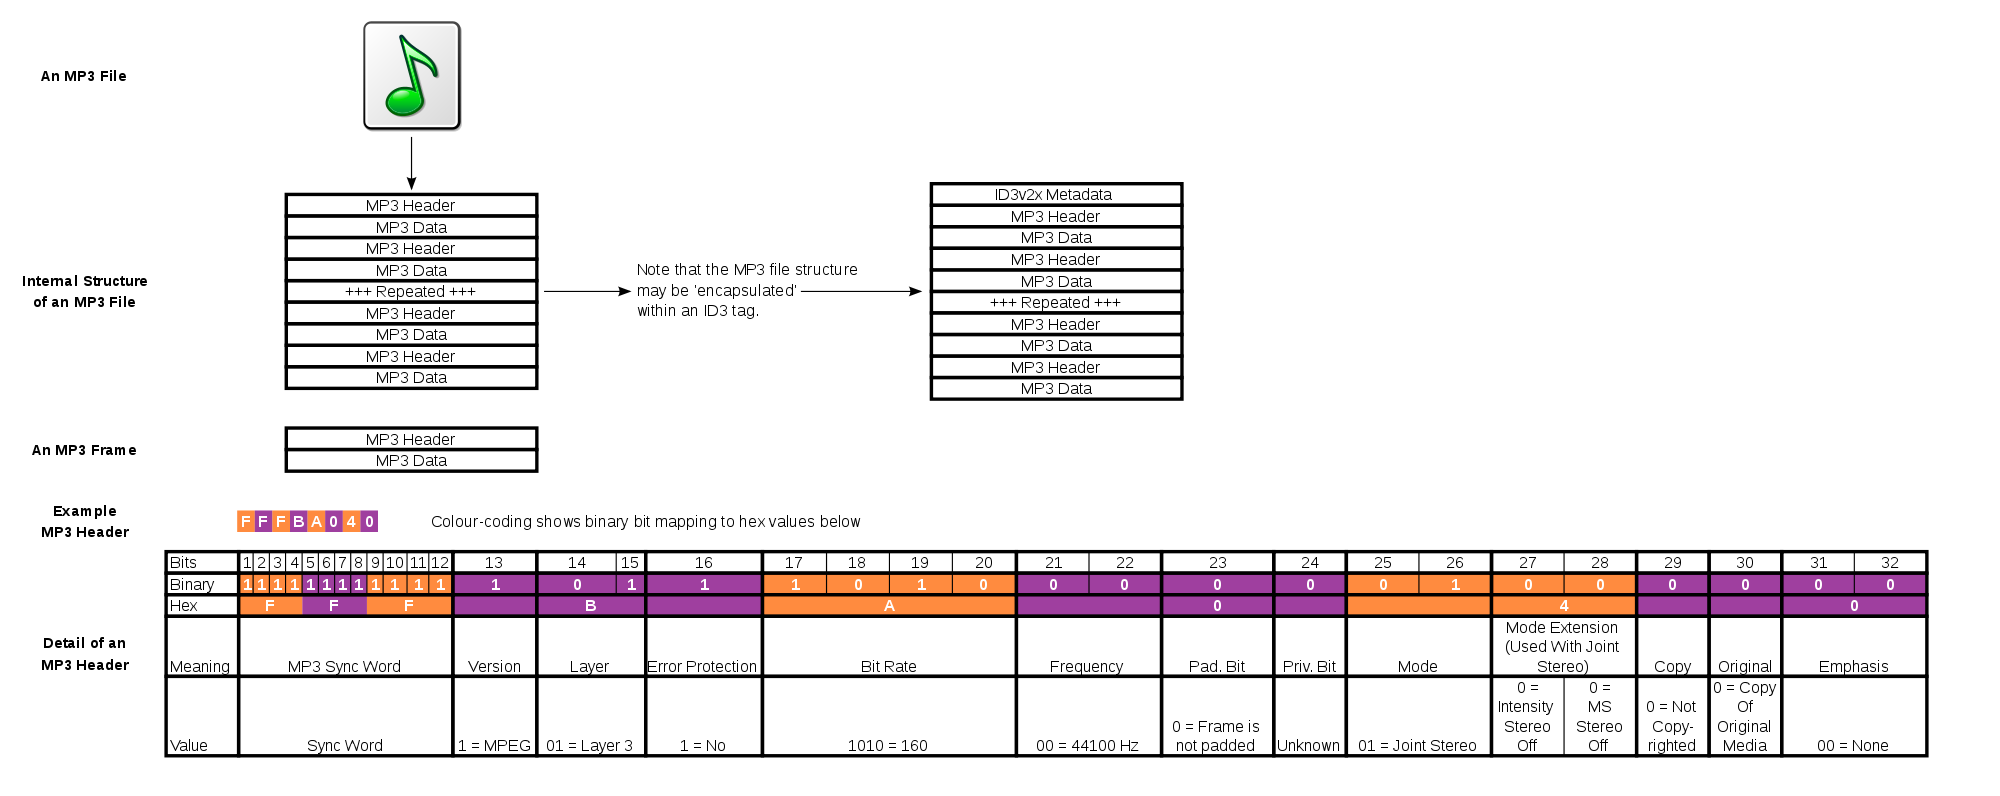
\includegraphics[width=1.1\textwidth]{1000px-Mp3filestructure}
  \caption{The mp3 header taken from wikipedia \cite{mike}}
\end{figure}
            \begin{itemize}
                \item{12 bits} All ones, sync word.
                \item{3 bits} 101 for MPEG layer 3.
                \item{1 bit} 0 if CRC follows the frame.
                \item{4 bits} Bitrate index.
                \item{2 bits} Sample rate index.
                \item{1 bit} 1 if frame is padded.
                \item{1 bit} Private bit - not used.
                \item{2 bits} Mode - Mono/Stereo/DualChannel/JointStereo.
                \item{2 bits} Mode extension - only used with JointStereo.
                \item{2 bits} Copyright data.
                \item{2 bits} Emphasis.
            \end{itemize}

            There are lots of data here that does not matter for the decoding
            process, and some that does not matter because of limits in our
            decoder. We restricted our decoder to files not using Joint Stereo,
            so the Mode Extension bits are not used. All bits are however
            checked for correctness. The most important bits for decoding are
            bitrate index (BT) and sample rate index (SR).

            The decoding process can be divided into two parts: unpacking and
            decoding. For the unpacking, the CRC info and padding data are also
            important.

            One might think that the header would contain all data needed for
            decoding, but that is absolutely not the case. In fact, the only
            useful data for decoding that is contained in the header are SR and
            BT. Then some data in the header is of course useful for unpacking,
            but unpacking is a rather small part of the whole decoding process.

       \subsubsection{Side Info}
            The side info is the part that contains most information on how to
            unpack the compressed audio and some information on how to decode
            the data. However, there is some information usable for decoding
            that is \textit{not} included in the side info, for some unknown
            reason. Some things to note in this data are:
            \begin{itemize}
                \item main\_data\_begin - a pointer to the audio data
                \item scfsi bands - scale factor information for each data part.
                \item part2\_3\_length - the amount of audio data for each
                      data part.
            \end{itemize}
            The rest of this section contains only decoding-specific data, which
            we will cover more in the implementation part.

       \subsubsection{Main Data}
            The main data is further divided into two granules, which may be
            divided further, depending on the number of channels (1 or 2). For
            each of these data parts, the main data contains scale information
            for decoding, and huffman data.

        \subsubsection{ID3}
            ID3 tags may be present within an mp3 file. Technically, it may
            appear anywhere in the file, but is by convention always in the
            beginning. Our decoder ignores id3 tags, however a library for
            parsing these tags was written for future use.

       \subsubsection{Other implementations}
           As earlier mention there exist several mp3 decoder
           implementations in various langugages such as C, Java, C++
           and also in Haskell (lame \cite{lame}, mad \cite{mad},
           LAMEOnJ \cite{lameonj}, Bjorns haskell mp3
           decoder \cite{bjorn}). The implementations made for other languages can
           decode in real time, but no such implementation exist in
           haskell yet. They all include a number of different
           optimizations for the heavy operations such as IMDCT,
           float calculations etc. that should be considered during
           this project. The existing implementation from Bjorn is
           only made to show how mp3 decoding is done and did not
           focus on being usable, which made his decoder easy to read
           and understand.

\section{Implementation}
    We wanted different parts of the process to be separate in the code, so we
    divided the decoder into two main modules: \texttt{Unpack.hs} and
    \texttt{Decode.hs}.

    \subsection{Unpacking}
\begin{figure}[h]
  \begin{center}
    \begin{lstlisting}
unpackMp3 :: L.ByteString -> [SideInfo BS.BitString]
unpackMp3 = runBitGet first . BS.convert
    where first = do
            skipId3
            init <- lookAhead (runMaybeT readHeader)
            unpackFrames init
    \end{lstlisting}
    \caption{Unpacking mp3}\label{fig:unpacking_mp3}
  \end{center}
\end{figure}

    What is going on here? The function expects a lazy \texttt{ByteString} as
    input (this is the contents of the mp3 file), and finally gives us a list of
    \texttt{SideInfo} datatypes parametrized by a \texttt{BitString}. There are
    lots of stuff that needs to be explained, clearly!

    First, what is the \texttt{SideInfo} type?
\begin{figure}[h]
  \begin{center}
    \begin{lstlisting}
data SideInfo a
    = Single { sampleRate  :: !Int
             , dataPointer :: !Int -- 9 bits
             , scales      :: ![Bool]
             , gran        :: !(Granule a, Granule a)
             }
    | Dual   { sampleRate  :: !Int
             , dataPointer :: !Int -- 9 bits
             , scales' :: ![Bool]
             , gran0  :: !(Granule a, Granule a)
             , gran1  :: !(Granule a, Granule a)
             } deriving Show
    \end{lstlisting}
    \caption{The SideInfo structure.}\label{fig:sideinfo_struct}
  \end{center}
\end{figure}

    So, it holds some values (\texttt{sampleRate}, \texttt{dataPointer}), some
    scale data information, and two or four \textit{granules}. There is a type
    of headers aswell, but that is only used intermediately when unpacking, so
    it is of rather little interest. We might describe it later.

    What is a \texttt{Granule} then? This is where the good stuff is!
\begin{figure}[h]
  \begin{center}
    \begin{lstlisting}
data Granule a = Granule {
    bigValues         :: !Int
  , globalGain        :: !Double
  , scaleFacCompress  :: !Int
  , windowSwitching   :: !Bool
    -- windows
  , blockType       :: !Int
  , mixedBlock      :: !Bool
  , tableSelect_1   :: !Int
  , tableSelect_2   :: !Int

    -- window == 0
  , tableSelect_3   :: !Int

    -- window == 1
  , subBlockGain1   :: !Double
  , subBlockGain2   :: !Double
  , subBlockGain3   :: !Double

  , preFlag           :: !Bool
  , scaleFacScale     :: !Bool
  , count1TableSelect :: !Bool

  -- calculated from previous values
  , region0Start     :: !Int
  , region1Start     :: !Int
  , region2Start     :: !Int

  , mp3Data          :: a
} deriving Show
    \end{lstlisting}
    \caption{A Granule at it's best}\label{fig:granule_type}
  \end{center}
\end{figure}

    The granule contains lots of information on how to decode, and then it
    contains an \texttt{a}. Recall that the result from \texttt{unpackMp3} was
    parametrized by a \texttt{BitString}, so the \texttt{mp3Data} in the granule
    would be a \texttt{BitString} in this case, holding the actual data to be
    decoded. \texttt{BitString} is a library we wrote during the project. It
    works like \texttt{ByteString}, but has support for bit-level operations,
    hence the name. We will cover \texttt{BitString} in section
    \ref{sec:bitstring}.

    We saw in \texttt{unpackMp3} that it read one frame, and then called
    \texttt{unpackFrames} with that frame as an argument. \texttt{unpackFrames}
    simply loops and accumulates frames until there are no more frames to read.
    The interesting function here is \texttt{readHeader}, which looks as
    follows:
\begin{figure}[h]
  \begin{center}
    \begin{lstlisting}
readHeader :: MaybeT BitGet (MP3Header Int)
readHeader = do
    h <- lift syncWord
    if not h then fail "" else do
        prot  <- lift $ liftM not getBit
        brate <- getBitRate
        freq  <- getFreq
        padd  <- lift getBit
        lift $ skip 1 -- private bit
        mode  <- getMode
        mext' <- getModeExt
        lift $ skip 4 -- copyright, original & emphasis
        when prot $ lift $ skip 16
        sinfo <- lift $ readSideInfo mode freq
        let size = ((144 * 1000 * brate) `div` freq +
                    if padd then 1 else 0) * 8
            f' = if prot then 2 else 0
            ff = case mode of
                Mono -> 17
                _    -> 32
            hsize = (f' + ff + 4) * 8
            mext = case mode of
                JointStereo -> mext'
                _ -> (False, False)
        return $ MP3Header mode mext size hsize sinfo
    \end{lstlisting}
    \caption{Reading the mp3 header}\label{fig:read_mp3_header}
  \end{center}
\end{figure}

    So, comparing it to the description of an mp3 header in section
    \ref{sec:header} we see that the only change is the size variable, which
    calculates the length in bits to the next header. This function however,
    does not read in any data, and thus does not produce a logical frame. To do
    that, we need to first read side info and then look ahead to the next
    header in order to determine how long we should read. The function that
    reads the data can be found in the source code of \texttt{Unpack.hs}, we do
    not include it here. However, we do include \texttt{readSideInfo}, since it
    is by far more interesting even though it is long.

\begin{figure}[h]
  \begin{center}
    \begin{lstlisting}
readSideInfo :: MP3Mode -> Int -> BitGet (SideInfo Int)
readSideInfo mode freq = do
    dataptr <- getInt 9
    skipPrivate
    scaleFactors <- getScaleFactors
    case mode of
        Mono -> do
            g0 <- getGranule
            g1 <- getGranule
            return $ Single freq (dataptr * 8)
                     scaleFactors (g0, g1)
        _    -> do
            g0 <- getGranule
            g1 <- getGranule
            g2 <- getGranule
            g3 <- getGranule
            return $ Dual freq (dataptr * 8)
                          scaleFactors (g0, g2) (g1, g3)
  where ...
    \end{lstlisting}
    \caption{Reading the side information of an mp3 file}\label{fig:sideinfo}
  \end{center}
\end{figure}

    So, lots of stuff that is done here are \textit{not} mentioned in the
    standard, but is stuff that one have to magically know (or see in somebody
    else's code, like we did). However, this is what a granule looks like,
    except for the data that is read in as stated above. Most of the stuff here
    is of little interest from a programming point of view, however all of them
    are used when decoding. The variables named \texttt{reg\{0,1,2\}len} are a
    bit more interesting though, since they control the number of times one has
    to invoke the huffman decoder. These variables are used together with
    \texttt{tableSelect\{0,1,2\}} that tells the decoder which huffman table
    that was used when compressing the audio data.

    \subsection{Decoding}
    \subsubsection{Huffman}
    We have had two approaches to huffman decoding; binary trees, and lookup
    tables (arrays). The first approach was the most intuitive one in which we
    read one bit at a time, and walked the tree until we had read a whole code
    word and reached a leaf. This was rather elegant and the code for doing so
    was no more than $\sim$10 lines. On the downside, this approach was very
    slow, and at that time the huffman decoder took almost 50\% of the total
    running time. We did some thinking, and looking at other people's ideas we
    found out that one could make rather large tables of size $2^n$ in the
    largest code word. Of course this was not practical, since the longest code
    word in one of the huffman tables was 19 bits, so we ended up with a 13MB
    source code file which was impossible to compile. We did some further
    thinking at this point, and came up with another idea! How about if we fix
    some code word length for a table (say 8), and for those code words that
    were longer a new table was returned. For those code words that were
    shorter, these were padded with all possible combinations to make it of the
    right length. It might be easier to understand with an example!
\begin{figure}[h]
  \begin{center}
    \begin{tabular}{| l | l |}
        \hline
        Code Word & Value \\ \hline \hline
        1   & 5 \\
        000 & 7 \\
        001 & 3 \\
        010 & 2 \\
        0111  & 4 \\
        01101 & 1 \\
        01100 & 8 \\ \hline
    \end{tabular}
    \caption{A Huffman table}\label{fig:huffmantab}
  \end{center}
\end{figure}

    In this case, one might choose code word length three, which we will use in
    this example. The lookup table generated from this would look like this:
\begin{figure}[h]
  \begin{center}
    \begin{tabular}{| l | l |}
        \hline
        Code Word & Value \\ \hline \hline
        100 & 5 \\
        101 & 5 \\
        110 & 5 \\
        111 & 5 \\
        000 & 7 \\
        001 & 3 \\
        010 & 2 \\ \hline
        011 & \begin{tabular}{l | l}
                10 & 4 \\
                11 & 4 \\
                01 & 1 \\
                00 & 8 \\
              \end{tabular} \\ \hline
    \end{tabular}
    \caption{Another huffman table}\label{fig:huffmantab2}
  \end{center}
\end{figure}

    So what happened here was that the one was expanded to fill all code words
    of length three starting with a one. The words that were of length three
    already were left as is, but the ones longer had one common factor of size
    three, 011. So if one reads 011, a new table is returned, where all code
    words are expanded to the longest one (two in this case). We see already
    here that this is much smaller than having $2^5$ entries (we have almost a
    three-fold in size here). With this approach, we could read more than one
    bit at the time. What we did was to read the common code word length number
    of bits. This saved time both in reading, and it saved us the traversal of a
    data structure, since it was replaced with an array lookup. Together with
    some other optimizations we lowered the amount of time taken by the huffman
    decoder to $\sim$8\%.

    \subsubsection{Audio Decoding}
        All audio is represented as floating-point numbers. Now, representing
        floats in a binary file format is not very space efficient, so the
        huffman decoder decodes integers instead of floats. These integers then
        has to be \textit{requantized}. \\

        At this point we were starting to get low on time. A lot of time had
        gone to parse the format and to huffman decode, largely due to the
        rather unspecific specification in ISO 11172-3. Therefore, some of the
        parts below will not be very well described, basically because we did
        not have time to investigate in how they work. Also, we will not show
        much of this code, since we did not write it. \\

        So, the \textit{requantization} is basically a transformation of all
        integers decoded by the huffman decoder into floats. How this is done
        depends on blocktype and windowswitching. Depending on those, different
        tables are for obtaining values that are multiplied by the integer from
        huffdecoding and also multiplied by different other more or less special
        values depending on blocktype and windowswitching. \\

        Next processing step is the reordering. During encoding, some parts of
        the data may be reordered in order to increase compression. The
        reordering basically reverses this process so that the actual audio is
        correctly ordered. Whenever the granule only has long blocks, this
        reordering is skipped. In the code, this step also pads the list of
        samples so that it is always of length 576 for simplicity in the further
        steps. \\

        To further compress the audio, the encoder passes the data through an
        \textit{Inverse Modified Discrete Cosine Transform} (IMDCT). As stated
        in ISO 11172-3, the transformation for each sample is done as
        follows:
\begin{figure}[h]
  \begin{center}
        \[
            x_i = \sum_{k=0}^{\frac{n}{2} - 1}{X_k * cos(\frac{\pi}{2n}(2i + 1 +
                  \frac{n}{2})(2k + 1))}
            \textit{ for i=0 to n-1}
        \]
    \caption{The IMDCT algorithm}\label{fig:imdctalgo}
  \end{center}
\end{figure}

        In the code that we plugged in to, the IMDCT was written as a piece of C
        code, as was the synthethis filterbank. We thought that it would be much
        nicer to have that code written in Haskell, so we rewrote both those
        files into Haskell versions. For the IMDCT that went extremely
        smooth:
\begin{figure}[h]
  \begin{center}
        \begin{lstlisting}
-- Straightforward translation from the C code.
imdct :: Int -> [Double] -> [Double]
imdct 18 xs  = imdct18 xs
imdct pts xs = map
    (\n -> sum $ zipWith (subone n) xs [0..pts-1])
    [0..2*pts-1]
  where
    subone :: Int -> Double -> Int -> Double
    subone n y k = y * (cos $ pipts
                            * (fi n + 0.5 + nhalf)
                            * (fi k + 0.5)
                       )
    pipts        = pi / (fi pts)
    nhalf        = (fi pts) / 2.0
        \end{lstlisting}
    \caption{IMDCT in haskell!}\label{fig:imdcthaskell}
  \end{center}
\end{figure}

\begin{figure}[h]
  \begin{center}
        \begin{lstlisting}
-- Straightforward translation from the C code, elegant!
imdct18 :: [Double] -> [Double]
imdct18 xs = map (\s -> sumZip (*) xs s) lookupIMDCT
  where
    -- 36x18 matrix
    lookupIMDCT :: [[Double]]
    lookupIMDCT = [[ cos $ (pi / 18.0) * n * k
                   | k <- [0.5, 1.5 .. 17.5]]
                   | n <- [9.5, 10.5 .. 44.5]]

    -- Instead of specialize
    sumZip _ [] _ = 0
    sumZip _ _ [] = 0
    sumZip f (a:as) (b:bs)
        = let acc = (f a b)
          in acc `seq` acc + sumZip f as bs
        \end{lstlisting}
    \caption{The specialization for 36 samples IMDCT algorithm}\label{fig:imdctimpl36}
  \end{center}
\end{figure}

        As you can see, there is a special version when there are only 18
        samples to transform, and we have not investigated in how that code was
        written, but we just translated it to Haskell, which in our opinion went
        very well. For performance reasons we wrote \texttt{sumZip}, which would
        not be needed otherwise. This was however quite slow compared to the C
        version, but that was not a big concern when we first wrote it, the goal
        was to have a Haskell version first, and if there were time, to
        optimise. \\

        The output of the IMDCT is inverted on all odd samples in odd sub bands,
        so they need to be inverted, in the code, this is done by simply
        changing the sign of them. \\

        The last step in the audio decoding is the synthethis filter bank, which
        when we plugged into the existing codec also was written in C, so it had
        to be rewritten in Haskell. This time however, it was not as neat as the
        IMDCT code. The synthethis filterbank was written in a far more
        imperative style, with lots and lots of array indexing, which made
        operations such as \texttt{map} and \texttt{zipWith} infeasible for this
        purpose. So this time we unfortunately had to write it in the same
        imperative style in Haskell as it was written in C, but with unboxed
        arrays in the \texttt{ST} monad.  Unlike the C version, we managed to
        separate the filterbank into two functions, one for updating the
        internal codec state, and one for computing the output.
        % TODO: Describe Synthethis more, maybe some code?

\section{Results}
    The result of this project is an mp3 decoder, written entirely in Haskell,
    that can decode an mp3 file, and output it to a file containing waveform
    audio. The decoder is very slow, decoding three minutes of audio takes
    approximately three minutes. The decoder has support for both Mono and
    Stereo, as well as Dual Channel, however Joint Stereo is not supported.

    \subsection{Discussion}
        Apart from the decoder being very slow, there are a number of things
        that could have been done differently, that may or may not have affected
        the speed of the decoder.

        Perhaps the first mistake we made was to assume that writing an mp3
        decoder would be just part of the project, when it in reality
        \textit{became} the project. If we would have known this from the start,
        more time could have been spent on working on the synthesis part. In
        relation to this, we feel that writing the parsing and unpacking parts
        took disproportionately much time in relation to the time it takes when
        running the decoder. We have both the mp3 standard and ourselves to
        blame for this; the mp3 standard for being unclear and fuzzy, and
        ourselves for not realising where we should have focused our work. 
        
        Us not realising focus might be due to us starting with the decoder that
        Björn had written, which meant that, for each step, we could see if we
        had done it right, just by jacking in our code in the appropriate parts
        of Björn's encoder. This had as effect that we went rather far in the
        project before we realised that we needed to write a back-end as well.

    \subsection{bitstring}
    \label{sec:bitstring}
        Initially, we started to parse the format using \texttt{ByteStrings},
        but since the MP3 format does not only deal in single bytes, but rather
        in single bits, we found that it would not be feasible to keep track of
        the bits by hand. Therefore, we wrote our own library,
        \texttt{BitString}.

        The BitString structure itself is rather simple:
        Initially, we started to parse the format using \texttt{ByteStrings},
        but since the MP3 format does not only deal in single bytes, but rather
        in single bits, we found that it would not be feasible to keep track of
        the bits by hand. Therefore, we wrote our own library,
        \texttt{BitString}.

        The \texttt{BitString} structure itself is rather simple:
\begin{figure}[h]
  \begin{center}
        \begin{lstlisting}
data BitString = Empty
               | Chunk L.ByteString !Word8 !Word8 BitString
        \end{lstlisting}
    \caption{A bitstring at it's core}\label{fig:bitstring}
  \end{center}
\end{figure}

        If you have ever used lazy \texttt{ByteStrings}, you will notice that
        the data definition here is similar, but with two extra
        \texttt{Word8}'s. The first is used to keep track of at which bit we are
        in the first byte, and the second one is used for knowing at which bit
        in the last byte the string ends (since \texttt{BitStrings} does not
        need to be full bytes). \\ The further design of the \texttt{BitString}
        library looks more or less like the \texttt{ByteString} library, but
        with additional functions for fetching bits, such as \texttt{takeWord8},
        \texttt{takeWord16} and so on. \\

        To make this library usable, we wanted to be able to operate on these
        \texttt{BitStrings} without keeping track of everything by ourselves,
        therefore we put it in a monad. This is how it looks:

\begin{figure}[h]
  \begin{center}
        \begin{lstlisting}
newtype BitGetT m a = BitGetT {
    unGet :: BitString -> m (a, BitString)
}
type BitGet = BitGetT Identity
instance (Monad m) => Monad (BitGetT m) where
    return a = BitGetT $ \bs -> return (a,bs)
    bg >>= f = BitGetT $ \bs -> do
        ~(a,bs') <- unGet bg bs
        unGet (f a) bs'
    \end{lstlisting}
    \caption{The bitstring monad}\label{fig:bitstringmonad}
  \end{center}
\end{figure}

    Much of the design of the \texttt{BitGet} monad was inspired by the existing
    \texttt{BitGet} monad available in the binary-strict package
    \cite{binarystrict}. However, it is not as extensive as the existing
    \texttt{BitGet} library, and it needs to include more handy functions before
    being released. Currently, we have only included functions that were needed
    for parsing the MP3 format.

    \subsection{huffman}
    \label{sec:huffman}
        Initially, we wrote a nice (but extremely slow) library for huffman
        encoding and decoding. This library was later subsumed by the huffman
        code available in \texttt{HuffArrays.hs}. The initial idea was based on the
        ground theory behind huffman codes, to have a tree with codes, and to
        traverse it when looking for the code for a value. That proved to be
        much too slow, since it did not only had to read one bit at the time,
        but also carry a large datastructure. Therefore we wrote the new
        version, which utilizes statically compiled arrays of variable size, but
        where the lookup in an array is always done with a fixed number of bits
        for every tree. The initial idea was to have $2^n$ entries in each
        table, where n would be the maximum size of a code word in that table,
        but that instantly showed to be impossible, since the maximum code word
        length for some tables are 18 and 19, this led to the tables being 13MB
        large, and could not be compiled. We then had to compromise, so we let
        the trees have at most $2^{10}$ entries, and in the cases where there were
        code words that were larger than 10 bits, the result from a lookup in
        the table was another table. The not-so-intuitive data structure looks
        like this:
\begin{figure}[h]
  \begin{center}
        \begin{lstlisting}
-- SmallTable / Deep Table
type MP3Huffman a = Either (HuffArray a) (HuffDeep a)
-- plain lookup
type HuffArray a  = (Int, Array Int (Int, a))
-- Int is Code Word length
-- In the array there may be values or arrays
type HuffDeep a  = (Int, Array Int
                         (Either (Int,a) (HuffArray a))
                   )
        \end{lstlisting}
    \caption{Huffaray}\label{fig:huffarraycode}
  \end{center}
\end{figure}

        But the complicated structure aside, this works very well, ever though
        \texttt{HuffTables.hs} still takes more time to compile than any other
        module.  The lookup function looks like this:
\begin{figure}[h]
  \begin{center}
        \begin{lstlisting}
-- Lookup a value in the huffman array
lookupHuff :: Monad m => MP3Huffman a -> BitGetT m (Int,a)
lookupHuff huff = case huff of
    Left  (cw,arr) -> liftM (arr !) (f cw)
    Right (cw,arr) -> do
        i <- f cw
        case arr ! i of
            Left a           -> return a
            Right (cw',arr') -> do
                (l,a) <- liftM (arr' !) (f cw')
                return (cw+l,a)
  where
    f w | w <= 8  = liftM fromIntegral
                    (getAsWord8 $ fromIntegral w)
        | w <= 16 = liftM fromIntegral
                    (getAsWord16 $ fromIntegral w)
        \end{lstlisting}
    \caption{Looking up huffcodes}\label{fig:lookuphuff}
  \end{center}
\end{figure}

        The huffman encoder that we wrote has never been used, and judging by
        its poor performance, it never should be.

\section{Future Work}
    There are a number of things that could be done in order to make this
    decoder work as desired.

    \subsection{Mutable structure}
        Large parts of the back-end currently uses an approach where data is
        transformed by functions having lists as arguments and having lists as
        results. Many parts of the back-end uses extensive list indexing, which
        becomes extremely slow with the current implementation. An interesting,
        but also style-breaking approach would be to use a mutable structure
        such as \texttt{STArray} or \texttt{IOArray}. This would make all code
        that uses list indexing work a lot faster, but much of the code would
        have to be rewritten to fit a more imperative style of programming,
        which would be unfortunate.

        Much work here could probably be done through more testing and
        optimisation, which we did not have time to do within the time scope of
        the project. Doing this both by looking at the existing code, and by
        examining the meaning of what the standard actually says would be
        helpful here.

    \subsection{Support for more mp3 modes}
        Currently, the decoder only has support for mono and stereo modes,
        whereas the standard also describes joint stereo, which is used in many
        mp3 encoders. It might be good to know that doing this would have impact
        on nearly every part of the decoder, since the different modes are both
        unpacked and decoded in different ways.

    \subsection{Back-end rewrite}
        The currently used back-end is mostly a rewrite of the back-end that
        Björns decoder uses. Since it was not written to be neither fast or
        efficient, we think that looking at other decoders such as madplay or
        ffmpeg would give good ideas for new algorithms in the decode phase.

    \subsection{Another huffman library}
        The huffman library we wrote turned out to never be used in the actual
        decoder due to its poor performance. Even though it is not really part
        of the project, it would be nice to create a new library based on the
        findings we did in this project.

    \subsection{The bitstring library}
        Apart from the actual decoder, the \texttt{bitstring} library is likely
        to be the most useful result from it. Actually, given the decoders
        current state, it is probably more useful. It is however not finished,
        and currently only consists of some very basic functions and functions
        that were needed in the decoder. Before the library can be released to
        the public we need to add more general functions to it. Actually, since
        we last coded on this project, a \texttt{bitstring} library has been
        released at Hackage by Balasz Komuves\cite{bitstring}, using another
        approach.

\begin{thebibliography}{99}
    \bibitem{bjorn}
        Let's build an MP3-decoder!
        http://blog.bjrn.se/2008/10/lets-build-mp3-decoder.html
    \bibitem{wikimp3}
        Wikipedia on MP3: http://en.wikipedia.org/wiki/Mp3
    \bibitem{wikimpeg1}
        Wikipedia on MPEG-1: http://en.wikipedia.org/wiki/MPEG-1
    \bibitem{binarystrict}
        Binary-Strict package on Hackage:
        http://hackage.haskell.org/package/binary-strict
    \bibitem{standard}
        ISO-11172-3 Information technology -- Coding of moving pictures and
        associated audio for digital storage media at up to about 1,5 Mbit/s --
        Part 3: Audio
    \bibitem{bitstring}
        Bitstring package on hackage:
        http://hackage.haskell.org/package/bitstring
     \bibitem{lameonj}
       LAMEOnJ
       http://openinnowhere.sourceforge.net/lameonj/
     \bibitem{mad}
       Mad
       http://www.underbit.com/products/mad/
     \bibitem{lame}
       LAME
       http://lame.sourceforge.net/
     \bibitem{mike}
       Kim Meyrick
       http://en.wikipedia.org/wiki/User:Kim\_Meyrick
\end{thebibliography}

\end{document}
